\documentclass[14pt]{extbook}
\usepackage{multicol, enumerate, enumitem, hyperref, color, soul, setspace, parskip, fancyhdr} %General Packages
\usepackage{amssymb, amsthm, amsmath, latexsym, units, mathtools} %Math Packages
\everymath{\displaystyle} %All math in Display Style
% Packages with additional options
\usepackage[headsep=0.5cm,headheight=12pt, left=1 in,right= 1 in,top= 1 in,bottom= 1 in]{geometry}
\usepackage[usenames,dvipsnames]{xcolor}
\usepackage{dashrule}  % Package to use the command below to create lines between items
\newcommand{\litem}[1]{\item#1\hspace*{-1cm}\rule{\textwidth}{0.4pt}}
\pagestyle{fancy}
\lhead{Progress Quiz 9}
\chead{}
\rhead{Version ALL}
\lfoot{9541-5764}
\cfoot{}
\rfoot{Summer C 2021}
\begin{document}

\begin{enumerate}
\litem{
Solve the quadratic equation below. Then, choose the intervals that the solutions $x_1$ and $x_2$ belong to, with $x_1 \leq x_2$.\[ 20x^{2} -81 x + 81 = 0 \]\begin{enumerate}[label=\Alph*.]
\item \( x_1 \in [0.67, 0.8] \text{ and } x_2 \in [5.39, 5.97] \)
\item \( x_1 \in [35.85, 36.16] \text{ and } x_2 \in [43.26, 46.08] \)
\item \( x_1 \in [1.78, 1.98] \text{ and } x_2 \in [2, 3.05] \)
\item \( x_1 \in [0.55, 0.68] \text{ and } x_2 \in [5.91, 7.68] \)
\item \( x_1 \in [0.29, 0.56] \text{ and } x_2 \in [8.36, 9.44] \)

\end{enumerate} }
\litem{
Write the equation of the graph presented below in the form $f(x)=ax^2+bx+c$, assuming  $a=1$ or $a=-1$. Then, choose the intervals that $a, b,$ and $c$ belong to.
\begin{center}
    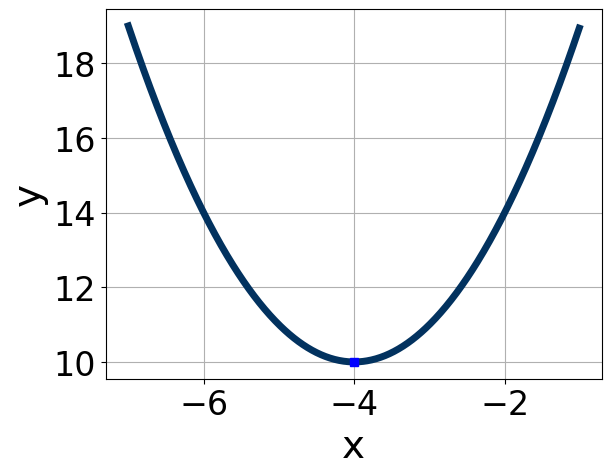
\includegraphics[width=0.5\textwidth]{../Figures/quadraticGraphToEquationA.png}
\end{center}
\begin{enumerate}[label=\Alph*.]
\item \( a \in [-0.1, 1.3], \hspace*{5mm} b \in [-9, -6], \text{ and } \hspace*{5mm} c \in [3, 8] \)
\item \( a \in [-0.1, 1.3], \hspace*{5mm} b \in [2, 11], \text{ and } \hspace*{5mm} c \in [25, 28] \)
\item \( a \in [-0.1, 1.3], \hspace*{5mm} b \in [-9, -6], \text{ and } \hspace*{5mm} c \in [25, 28] \)
\item \( a \in [-1.2, 0.3], \hspace*{5mm} b \in [-9, -6], \text{ and } \hspace*{5mm} c \in [-7, -3] \)
\item \( a \in [-1.2, 0.3], \hspace*{5mm} b \in [2, 11], \text{ and } \hspace*{5mm} c \in [-7, -3] \)

\end{enumerate} }
\litem{
Graph the equation below.\[ f(x) = (x-3)^2 - 16 \]\begin{enumerate}[label=\Alph*.]
\begin{multicols}{2}\item 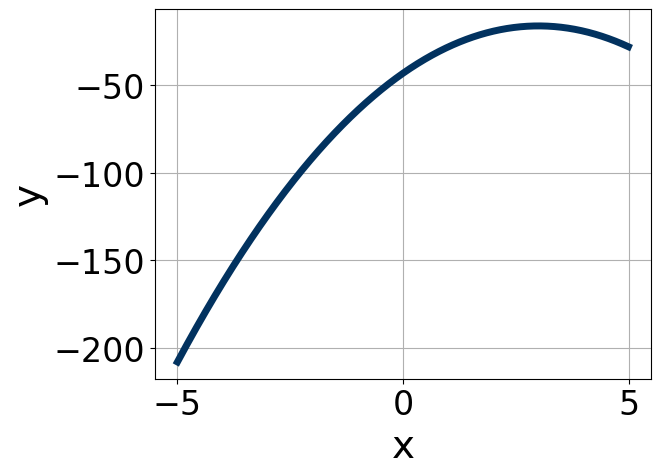
\includegraphics[width = 0.3\textwidth]{../Figures/quadraticEquationToGraphCopyAA.png}\item 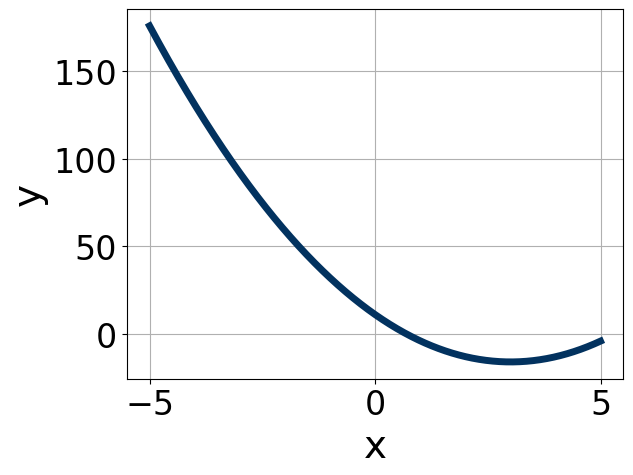
\includegraphics[width = 0.3\textwidth]{../Figures/quadraticEquationToGraphCopyBA.png}\item 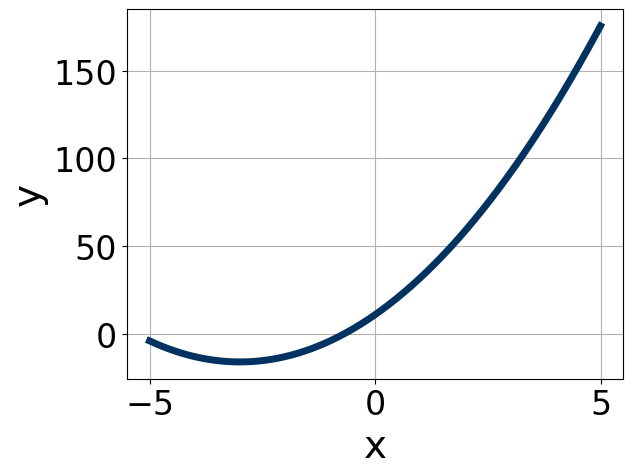
\includegraphics[width = 0.3\textwidth]{../Figures/quadraticEquationToGraphCopyCA.png}\item 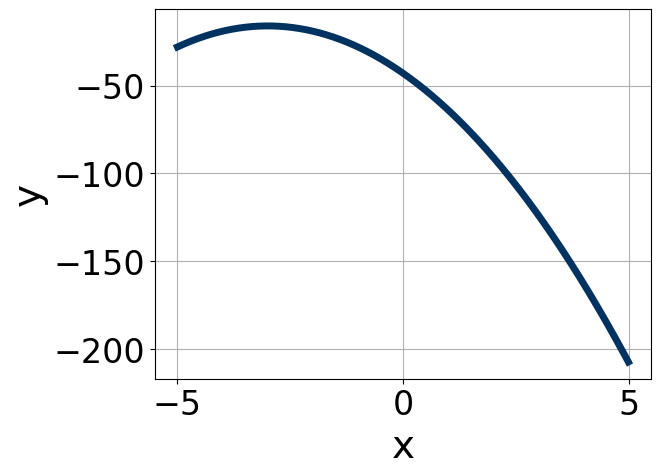
\includegraphics[width = 0.3\textwidth]{../Figures/quadraticEquationToGraphCopyDA.png}\end{multicols}\item None of the above.
\end{enumerate} }
\litem{
Graph the equation below.\[ f(x) = (x+3)^2 + 18 \]\begin{enumerate}[label=\Alph*.]
\begin{multicols}{2}\item 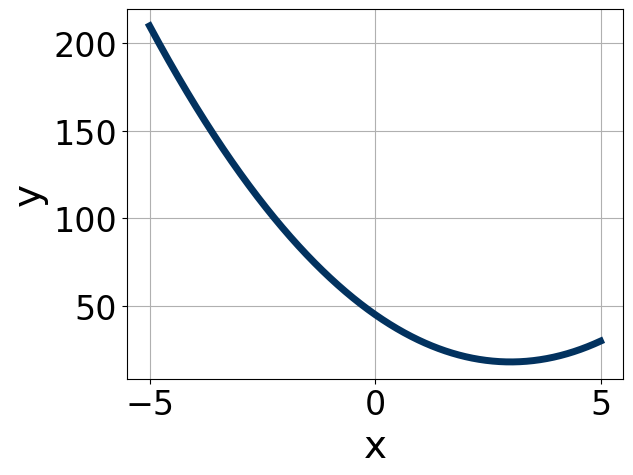
\includegraphics[width = 0.3\textwidth]{../Figures/quadraticEquationToGraphAA.png}\item 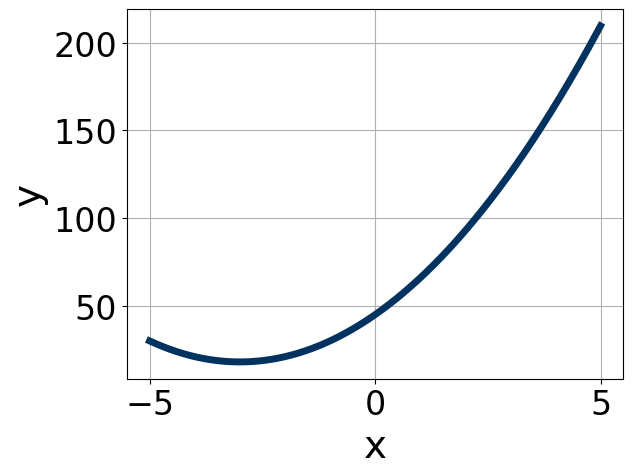
\includegraphics[width = 0.3\textwidth]{../Figures/quadraticEquationToGraphBA.png}\item 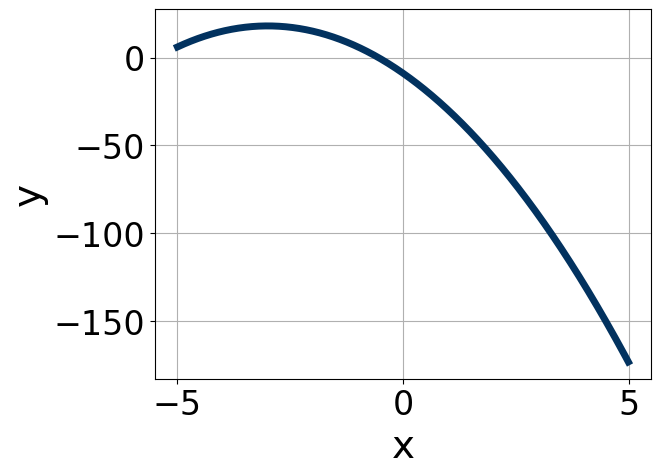
\includegraphics[width = 0.3\textwidth]{../Figures/quadraticEquationToGraphCA.png}\item 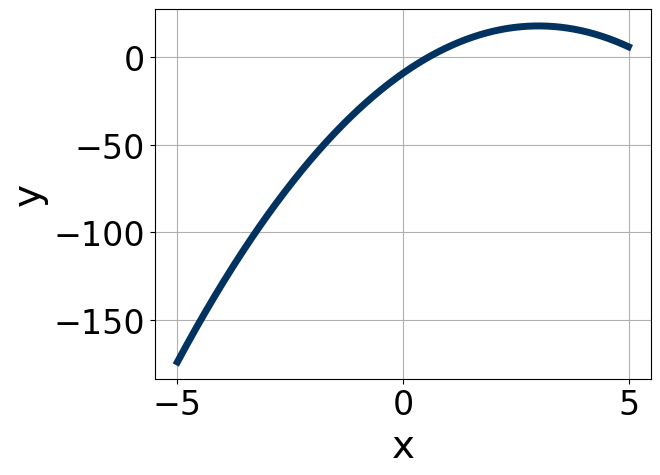
\includegraphics[width = 0.3\textwidth]{../Figures/quadraticEquationToGraphDA.png}\end{multicols}\item None of the above.
\end{enumerate} }
\litem{
Solve the quadratic equation below. Then, choose the intervals that the solutions $x_1$ and $x_2$ belong to, with $x_1 \leq x_2$.\[ 15x^{2} +32 x + 16 = 0 \]\begin{enumerate}[label=\Alph*.]
\item \( x_1 \in [-1.45, -0.81] \text{ and } x_2 \in [-0.89, -0.72] \)
\item \( x_1 \in [-20.22, -19.79] \text{ and } x_2 \in [-12.21, -11.95] \)
\item \( x_1 \in [-4.39, -3.78] \text{ and } x_2 \in [-0.39, -0.18] \)
\item \( x_1 \in [-2.77, -2.25] \text{ and } x_2 \in [-0.46, -0.34] \)
\item \( x_1 \in [-2.04, -1.51] \text{ and } x_2 \in [-0.67, -0.49] \)

\end{enumerate} }
\litem{
Solve the quadratic equation below. Then, choose the intervals that the solutions belong to, with $x_1 \leq x_2$ (if they exist).\[ 16x^{2} +11 x -8 = 0 \]\begin{enumerate}[label=\Alph*.]
\item \( x_1 \in [-1.2, -0.7] \text{ and } x_2 \in [-0.92, 0.61] \)
\item \( x_1 \in [-26.1, -24.8] \text{ and } x_2 \in [23.7, 25.07] \)
\item \( x_1 \in [-18.2, -17.6] \text{ and } x_2 \in [7.04, 7.33] \)
\item \( x_1 \in [-0.9, 1.3] \text{ and } x_2 \in [0.79, 1.41] \)
\item \( \text{There are no Real solutions.} \)

\end{enumerate} }
\litem{
Write the equation of the graph presented below in the form $f(x)=ax^2+bx+c$, assuming  $a=1$ or $a=-1$. Then, choose the intervals that $a, b,$ and $c$ belong to.
\begin{center}
    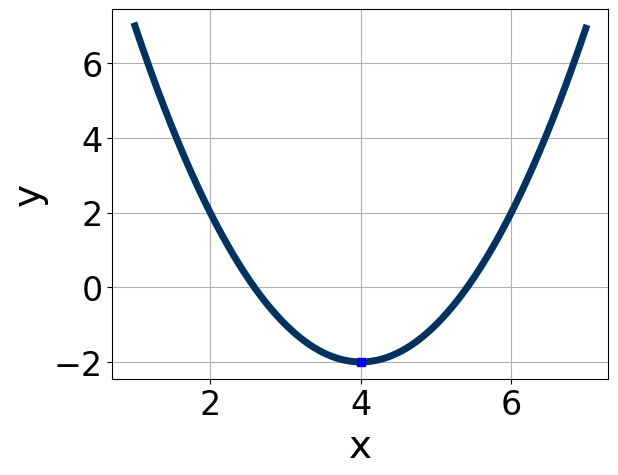
\includegraphics[width=0.5\textwidth]{../Figures/quadraticGraphToEquationCopyA.png}
\end{center}
\begin{enumerate}[label=\Alph*.]
\item \( a \in [-0.9, 1.7], \hspace*{5mm} b \in [-8, -5], \text{ and } \hspace*{5mm} c \in [13, 15] \)
\item \( a \in [-0.9, 1.7], \hspace*{5mm} b \in [6, 10], \text{ and } \hspace*{5mm} c \in [13, 15] \)
\item \( a \in [-2.4, 0.4], \hspace*{5mm} b \in [6, 10], \text{ and } \hspace*{5mm} c \in [-18, -16] \)
\item \( a \in [-2.4, 0.4], \hspace*{5mm} b \in [-8, -5], \text{ and } \hspace*{5mm} c \in [-18, -16] \)
\item \( a \in [-0.9, 1.7], \hspace*{5mm} b \in [6, 10], \text{ and } \hspace*{5mm} c \in [17, 20] \)

\end{enumerate} }
\litem{
Factor the quadratic below. Then, choose the intervals that contain the constants in the form $(ax+b)(cx+d); b \leq d.$\[ 54x^{2} +33 x -10 \]\begin{enumerate}[label=\Alph*.]
\item \( a \in [7.3, 9.9], \hspace*{5mm} b \in [-5, -1], \hspace*{5mm} c \in [5.9, 7.4], \text{ and } \hspace*{5mm} d \in [5, 7] \)
\item \( a \in [17.3, 18.2], \hspace*{5mm} b \in [-5, -1], \hspace*{5mm} c \in [1.9, 5.9], \text{ and } \hspace*{5mm} d \in [5, 7] \)
\item \( a \in [2.7, 4.3], \hspace*{5mm} b \in [-5, -1], \hspace*{5mm} c \in [16.7, 18.3], \text{ and } \hspace*{5mm} d \in [5, 7] \)
\item \( a \in [0.8, 1.1], \hspace*{5mm} b \in [-19, -7], \hspace*{5mm} c \in [-0.2, 1.9], \text{ and } \hspace*{5mm} d \in [41, 47] \)
\item \( \text{None of the above.} \)

\end{enumerate} }
\litem{
Factor the quadratic below. Then, choose the intervals that contain the constants in the form $(ax+b)(cx+d); b \leq d.$\[ 16x^{2} +32 x + 15 \]\begin{enumerate}[label=\Alph*.]
\item \( a \in [1.33, 2.64], \hspace*{5mm} b \in [1, 6], \hspace*{5mm} c \in [7.58, 8.67], \text{ and } \hspace*{5mm} d \in [0, 7] \)
\item \( a \in [3.49, 4.26], \hspace*{5mm} b \in [1, 6], \hspace*{5mm} c \in [2.79, 4.2], \text{ and } \hspace*{5mm} d \in [0, 7] \)
\item \( a \in [0.58, 1.65], \hspace*{5mm} b \in [11, 17], \hspace*{5mm} c \in [0.83, 1.1], \text{ and } \hspace*{5mm} d \in [19, 28] \)
\item \( a \in [7.94, 8.37], \hspace*{5mm} b \in [1, 6], \hspace*{5mm} c \in [1.14, 2.49], \text{ and } \hspace*{5mm} d \in [0, 7] \)
\item \( \text{None of the above.} \)

\end{enumerate} }
\litem{
Solve the quadratic equation below. Then, choose the intervals that the solutions belong to, with $x_1 \leq x_2$ (if they exist).\[ -18x^{2} -12 x + 7 = 0 \]\begin{enumerate}[label=\Alph*.]
\item \( x_1 \in [-1.49, -0.59] \text{ and } x_2 \in [-0.22, 0.88] \)
\item \( x_1 \in [-26.38, -25.01] \text{ and } x_2 \in [25.08, 26.1] \)
\item \( x_1 \in [-0.57, 0.29] \text{ and } x_2 \in [0.7, 2.14] \)
\item \( x_1 \in [-6.86, -6.62] \text{ and } x_2 \in [17.57, 18.78] \)
\item \( \text{There are no Real solutions.} \)

\end{enumerate} }
\litem{
Solve the quadratic equation below. Then, choose the intervals that the solutions $x_1$ and $x_2$ belong to, with $x_1 \leq x_2$.\[ 25x^{2} +75 x + 54 = 0 \]\begin{enumerate}[label=\Alph*.]
\item \( x_1 \in [-1.86, -1.47] \text{ and } x_2 \in [-1.31, -1.15] \)
\item \( x_1 \in [-46.12, -44.27] \text{ and } x_2 \in [-30.08, -29.85] \)
\item \( x_1 \in [-2.51, -2.32] \text{ and } x_2 \in [-1.13, -0.83] \)
\item \( x_1 \in [-5.87, -4.97] \text{ and } x_2 \in [-0.5, -0.33] \)
\item \( x_1 \in [-10.18, -7.05] \text{ and } x_2 \in [-0.31, -0.04] \)

\end{enumerate} }
\litem{
Write the equation of the graph presented below in the form $f(x)=ax^2+bx+c$, assuming  $a=1$ or $a=-1$. Then, choose the intervals that $a, b,$ and $c$ belong to.
\begin{center}
    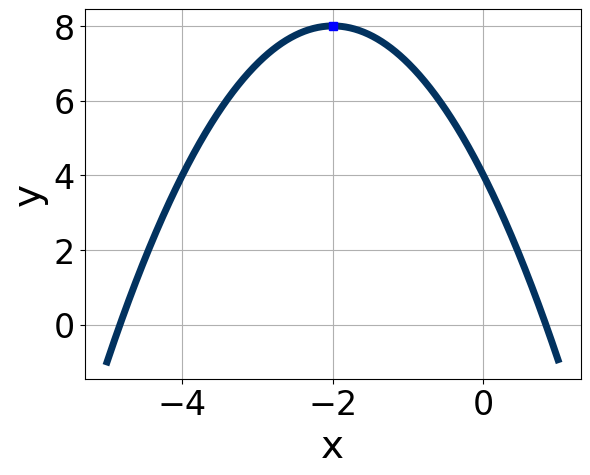
\includegraphics[width=0.5\textwidth]{../Figures/quadraticGraphToEquationB.png}
\end{center}
\begin{enumerate}[label=\Alph*.]
\item \( a \in [-2, 0], \hspace*{5mm} b \in [3, 8], \text{ and } \hspace*{5mm} c \in [4, 5] \)
\item \( a \in [-2, 0], \hspace*{5mm} b \in [3, 8], \text{ and } \hspace*{5mm} c \in [-12, -10] \)
\item \( a \in [-2, 0], \hspace*{5mm} b \in [-4, -1], \text{ and } \hspace*{5mm} c \in [4, 5] \)
\item \( a \in [0, 2], \hspace*{5mm} b \in [-4, -1], \text{ and } \hspace*{5mm} c \in [9, 14] \)
\item \( a \in [0, 2], \hspace*{5mm} b \in [3, 8], \text{ and } \hspace*{5mm} c \in [9, 14] \)

\end{enumerate} }
\litem{
Graph the equation below.\[ f(x) = -(x+1)^2 + 14 \]\begin{enumerate}[label=\Alph*.]
\begin{multicols}{2}\item 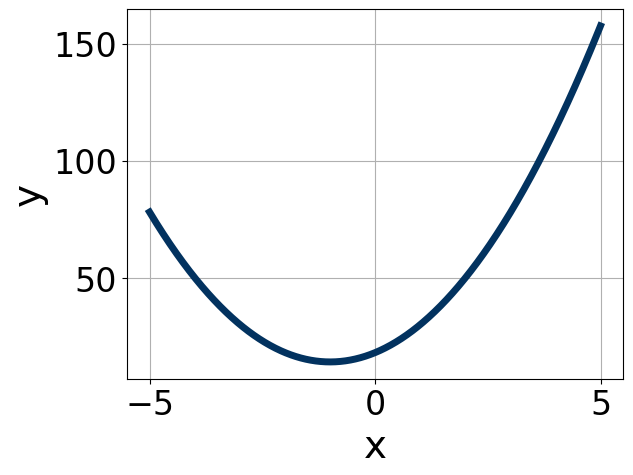
\includegraphics[width = 0.3\textwidth]{../Figures/quadraticEquationToGraphCopyAB.png}\item 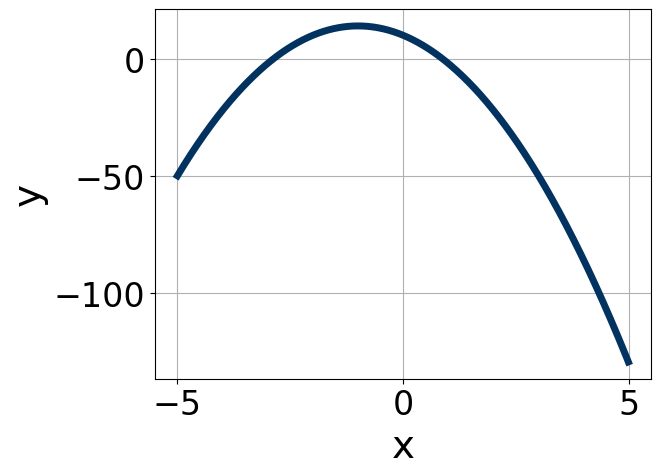
\includegraphics[width = 0.3\textwidth]{../Figures/quadraticEquationToGraphCopyBB.png}\item 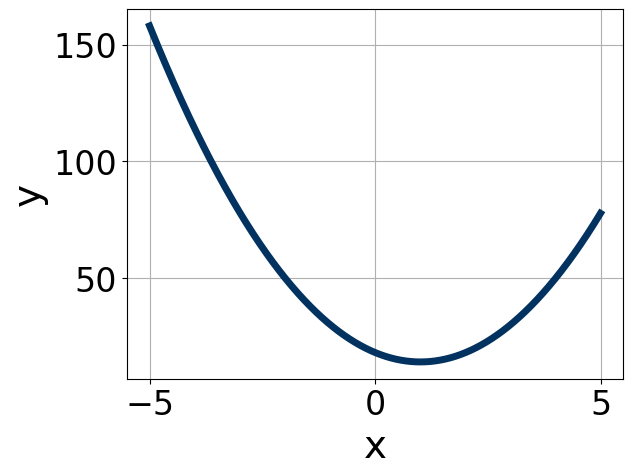
\includegraphics[width = 0.3\textwidth]{../Figures/quadraticEquationToGraphCopyCB.png}\item 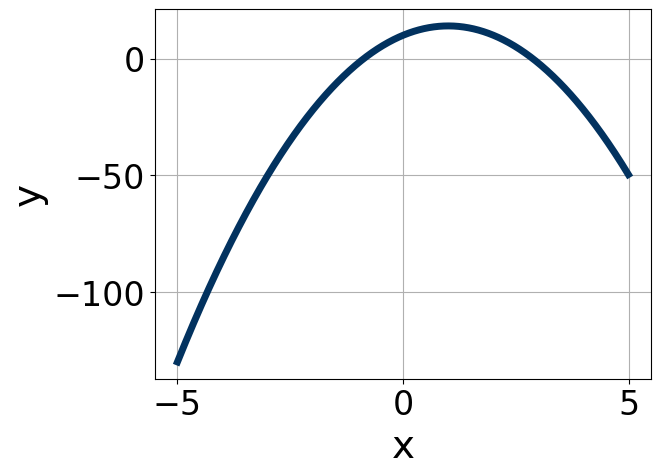
\includegraphics[width = 0.3\textwidth]{../Figures/quadraticEquationToGraphCopyDB.png}\end{multicols}\item None of the above.
\end{enumerate} }
\litem{
Graph the equation below.\[ f(x) = -(x+1)^2 + 12 \]\begin{enumerate}[label=\Alph*.]
\begin{multicols}{2}\item 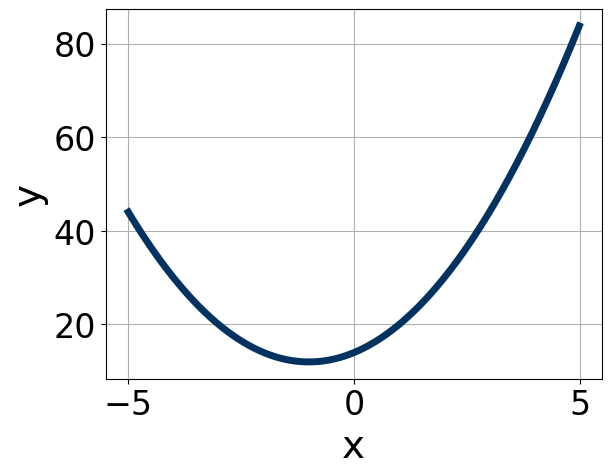
\includegraphics[width = 0.3\textwidth]{../Figures/quadraticEquationToGraphAB.png}\item 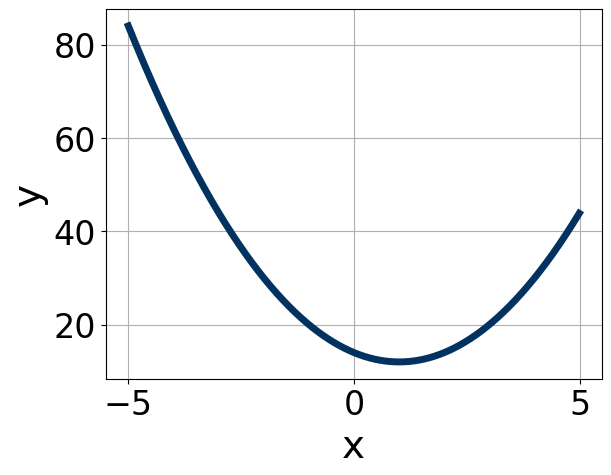
\includegraphics[width = 0.3\textwidth]{../Figures/quadraticEquationToGraphBB.png}\item 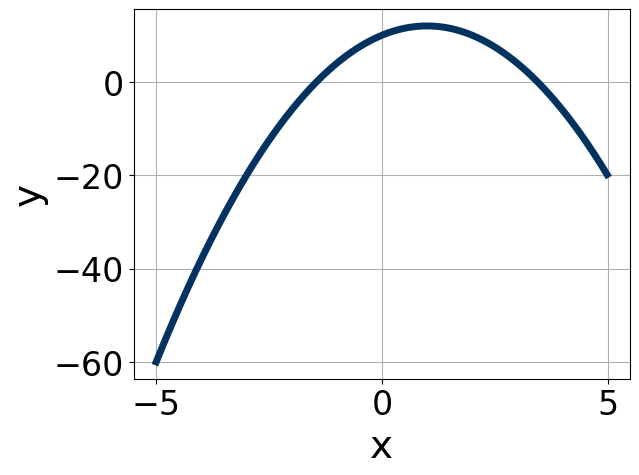
\includegraphics[width = 0.3\textwidth]{../Figures/quadraticEquationToGraphCB.png}\item 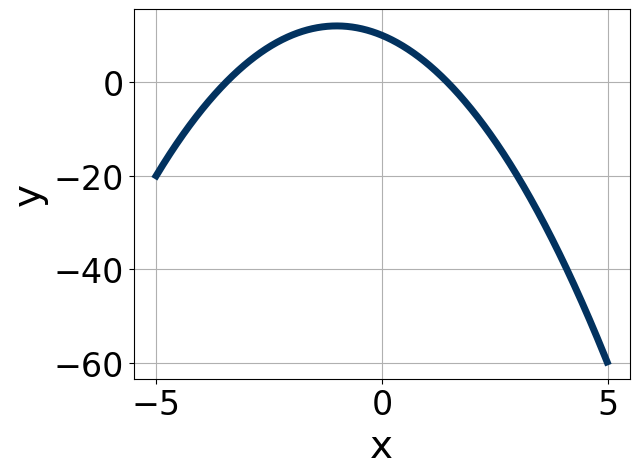
\includegraphics[width = 0.3\textwidth]{../Figures/quadraticEquationToGraphDB.png}\end{multicols}\item None of the above.
\end{enumerate} }
\litem{
Solve the quadratic equation below. Then, choose the intervals that the solutions $x_1$ and $x_2$ belong to, with $x_1 \leq x_2$.\[ 25x^{2} +50 x + 24 = 0 \]\begin{enumerate}[label=\Alph*.]
\item \( x_1 \in [-2.76, -1.62] \text{ and } x_2 \in [-0.44, -0.18] \)
\item \( x_1 \in [-30.33, -29.48] \text{ and } x_2 \in [-20.15, -19.54] \)
\item \( x_1 \in [-1.53, -0.44] \text{ and } x_2 \in [-1.02, -0.8] \)
\item \( x_1 \in [-6.4, -5.95] \text{ and } x_2 \in [-0.27, 0.26] \)
\item \( x_1 \in [-2.06, -1.47] \text{ and } x_2 \in [-0.79, -0.45] \)

\end{enumerate} }
\litem{
Solve the quadratic equation below. Then, choose the intervals that the solutions belong to, with $x_1 \leq x_2$ (if they exist).\[ -19x^{2} -14 x + 9 = 0 \]\begin{enumerate}[label=\Alph*.]
\item \( x_1 \in [-1.79, -0.99] \text{ and } x_2 \in [-0.31, 0.65] \)
\item \( x_1 \in [-30.36, -29.59] \text{ and } x_2 \in [29.26, 30.14] \)
\item \( x_1 \in [-8.31, -6.86] \text{ and } x_2 \in [21.46, 22.28] \)
\item \( x_1 \in [-1.06, 0.8] \text{ and } x_2 \in [0.92, 1.45] \)
\item \( \text{There are no Real solutions.} \)

\end{enumerate} }
\litem{
Write the equation of the graph presented below in the form $f(x)=ax^2+bx+c$, assuming  $a=1$ or $a=-1$. Then, choose the intervals that $a, b,$ and $c$ belong to.
\begin{center}
    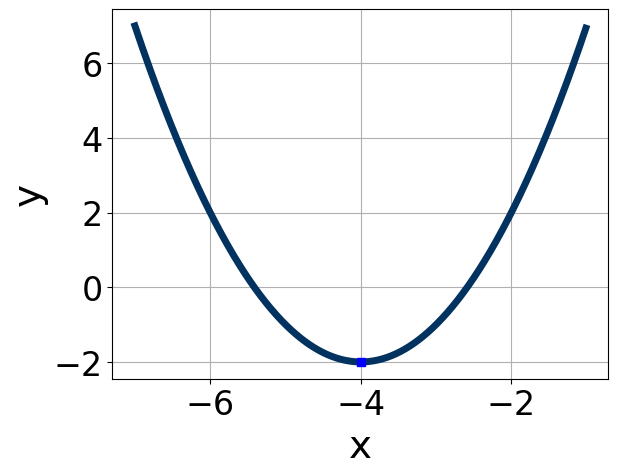
\includegraphics[width=0.5\textwidth]{../Figures/quadraticGraphToEquationCopyB.png}
\end{center}
\begin{enumerate}[label=\Alph*.]
\item \( a \in [-2.5, 0.6], \hspace*{5mm} b \in [-9, -7], \text{ and } \hspace*{5mm} c \in [-24, -15] \)
\item \( a \in [-2.5, 0.6], \hspace*{5mm} b \in [5, 12], \text{ and } \hspace*{5mm} c \in [-24, -15] \)
\item \( a \in [0.9, 1.5], \hspace*{5mm} b \in [-9, -7], \text{ and } \hspace*{5mm} c \in [13, 16] \)
\item \( a \in [0.9, 1.5], \hspace*{5mm} b \in [-9, -7], \text{ and } \hspace*{5mm} c \in [16, 22] \)
\item \( a \in [0.9, 1.5], \hspace*{5mm} b \in [5, 12], \text{ and } \hspace*{5mm} c \in [13, 16] \)

\end{enumerate} }
\litem{
Factor the quadratic below. Then, choose the intervals that contain the constants in the form $(ax+b)(cx+d); b \leq d.$\[ 24x^{2} -10 x -25 \]\begin{enumerate}[label=\Alph*.]
\item \( a \in [1.04, 2.41], \hspace*{5mm} b \in [-10, 0], \hspace*{5mm} c \in [10.5, 16.1], \text{ and } \hspace*{5mm} d \in [1, 9] \)
\item \( a \in [2.66, 5.06], \hspace*{5mm} b \in [-10, 0], \hspace*{5mm} c \in [5.6, 7.2], \text{ and } \hspace*{5mm} d \in [1, 9] \)
\item \( a \in [0.71, 1.26], \hspace*{5mm} b \in [-32, -28], \hspace*{5mm} c \in [-0.9, 2.2], \text{ and } \hspace*{5mm} d \in [20, 28] \)
\item \( a \in [6.55, 8.23], \hspace*{5mm} b \in [-10, 0], \hspace*{5mm} c \in [1.4, 4.5], \text{ and } \hspace*{5mm} d \in [1, 9] \)
\item \( \text{None of the above.} \)

\end{enumerate} }
\litem{
Factor the quadratic below. Then, choose the intervals that contain the constants in the form $(ax+b)(cx+d); b \leq d.$\[ 36x^{2} -60 x + 25 \]\begin{enumerate}[label=\Alph*.]
\item \( a \in [-2.7, 2.9], \hspace*{5mm} b \in [-31, -21], \hspace*{5mm} c \in [0.57, 1.73], \text{ and } \hspace*{5mm} d \in [-34, -27] \)
\item \( a \in [2.2, 5], \hspace*{5mm} b \in [-12, -3], \hspace*{5mm} c \in [11.82, 13.04], \text{ and } \hspace*{5mm} d \in [-5, -4] \)
\item \( a \in [5.7, 6.1], \hspace*{5mm} b \in [-12, -3], \hspace*{5mm} c \in [5.25, 6.79], \text{ and } \hspace*{5mm} d \in [-5, -4] \)
\item \( a \in [16.7, 20.6], \hspace*{5mm} b \in [-12, -3], \hspace*{5mm} c \in [1.01, 3.29], \text{ and } \hspace*{5mm} d \in [-5, -4] \)
\item \( \text{None of the above.} \)

\end{enumerate} }
\litem{
Solve the quadratic equation below. Then, choose the intervals that the solutions belong to, with $x_1 \leq x_2$ (if they exist).\[ 12x^{2} -14 x -3 = 0 \]\begin{enumerate}[label=\Alph*.]
\item \( x_1 \in [-18.81, -16.92] \text{ and } x_2 \in [17.6, 20.1] \)
\item \( x_1 \in [-1.89, -0.28] \text{ and } x_2 \in [-0.9, 0.6] \)
\item \( x_1 \in [-1.19, 0.7] \text{ and } x_2 \in [1, 2.7] \)
\item \( x_1 \in [-2.47, -1.62] \text{ and } x_2 \in [14.5, 16.9] \)
\item \( \text{There are no Real solutions.} \)

\end{enumerate} }
\litem{
Solve the quadratic equation below. Then, choose the intervals that the solutions $x_1$ and $x_2$ belong to, with $x_1 \leq x_2$.\[ 25x^{2} -60 x + 36 = 0 \]\begin{enumerate}[label=\Alph*.]
\item \( x_1 \in [0.54, 0.61] \text{ and } x_2 \in [1.77, 2.78] \)
\item \( x_1 \in [0.17, 0.35] \text{ and } x_2 \in [4.56, 6.52] \)
\item \( x_1 \in [29.74, 30.37] \text{ and } x_2 \in [29.71, 30.04] \)
\item \( x_1 \in [0.76, 1.75] \text{ and } x_2 \in [1.01, 1.77] \)
\item \( x_1 \in [0.37, 0.55] \text{ and } x_2 \in [3.25, 4.59] \)

\end{enumerate} }
\litem{
Write the equation of the graph presented below in the form $f(x)=ax^2+bx+c$, assuming  $a=1$ or $a=-1$. Then, choose the intervals that $a, b,$ and $c$ belong to.
\begin{center}
    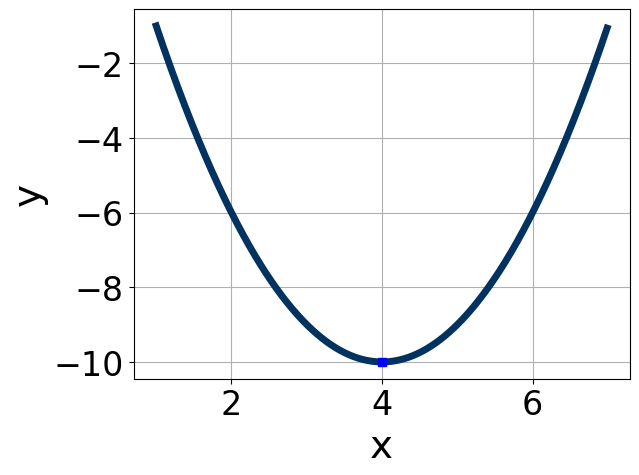
\includegraphics[width=0.5\textwidth]{../Figures/quadraticGraphToEquationC.png}
\end{center}
\begin{enumerate}[label=\Alph*.]
\item \( a \in [-1.8, -0.5], \hspace*{5mm} b \in [-10, -5], \text{ and } \hspace*{5mm} c \in [-26, -23] \)
\item \( a \in [0.7, 1.1], \hspace*{5mm} b \in [5, 11], \text{ and } \hspace*{5mm} c \in [6, 9] \)
\item \( a \in [-1.8, -0.5], \hspace*{5mm} b \in [5, 11], \text{ and } \hspace*{5mm} c \in [-26, -23] \)
\item \( a \in [0.7, 1.1], \hspace*{5mm} b \in [-10, -5], \text{ and } \hspace*{5mm} c \in [6, 9] \)
\item \( a \in [0.7, 1.1], \hspace*{5mm} b \in [5, 11], \text{ and } \hspace*{5mm} c \in [25, 27] \)

\end{enumerate} }
\litem{
Graph the equation below.\[ f(x) = -(x+1)^2 + 10 \]\begin{enumerate}[label=\Alph*.]
\begin{multicols}{2}\item 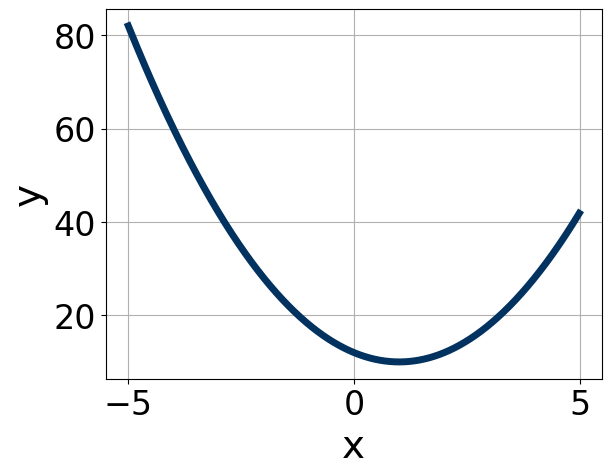
\includegraphics[width = 0.3\textwidth]{../Figures/quadraticEquationToGraphCopyAC.png}\item 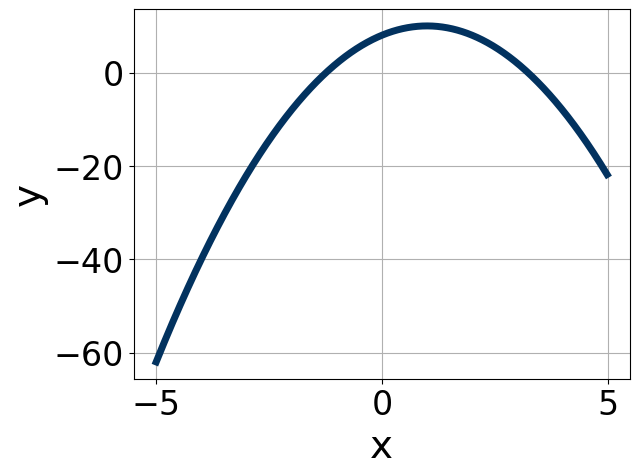
\includegraphics[width = 0.3\textwidth]{../Figures/quadraticEquationToGraphCopyBC.png}\item 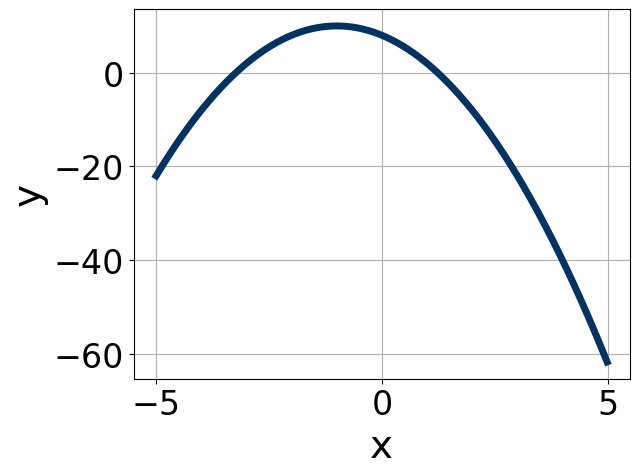
\includegraphics[width = 0.3\textwidth]{../Figures/quadraticEquationToGraphCopyCC.png}\item 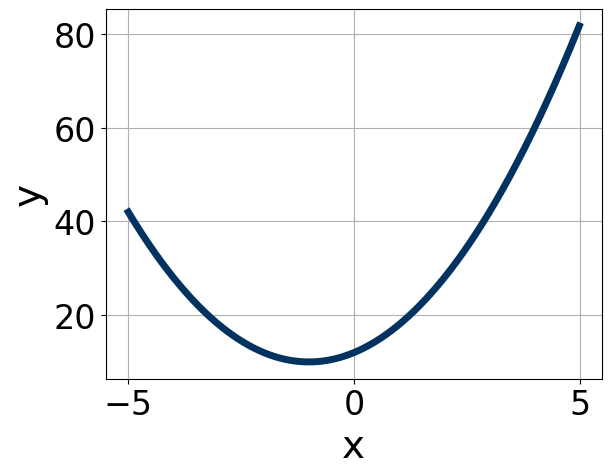
\includegraphics[width = 0.3\textwidth]{../Figures/quadraticEquationToGraphCopyDC.png}\end{multicols}\item None of the above.
\end{enumerate} }
\litem{
Graph the equation below.\[ f(x) = -(x+2)^2 + 11 \]\begin{enumerate}[label=\Alph*.]
\begin{multicols}{2}\item 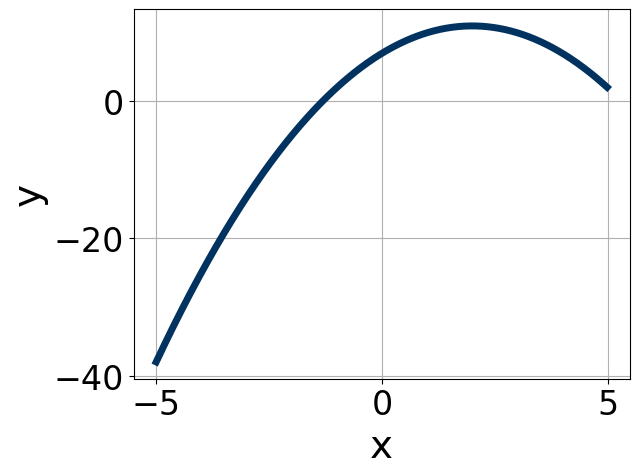
\includegraphics[width = 0.3\textwidth]{../Figures/quadraticEquationToGraphAC.png}\item 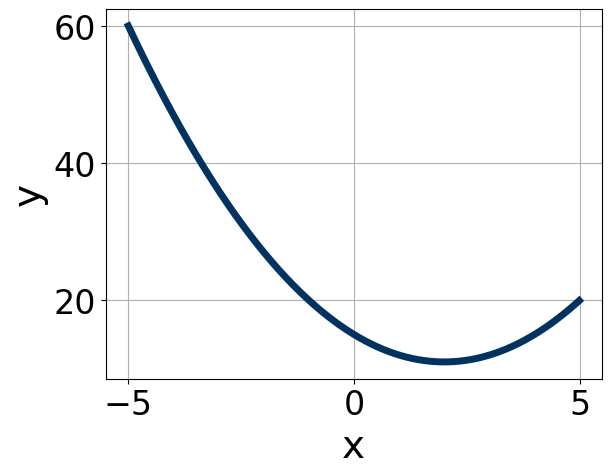
\includegraphics[width = 0.3\textwidth]{../Figures/quadraticEquationToGraphBC.png}\item 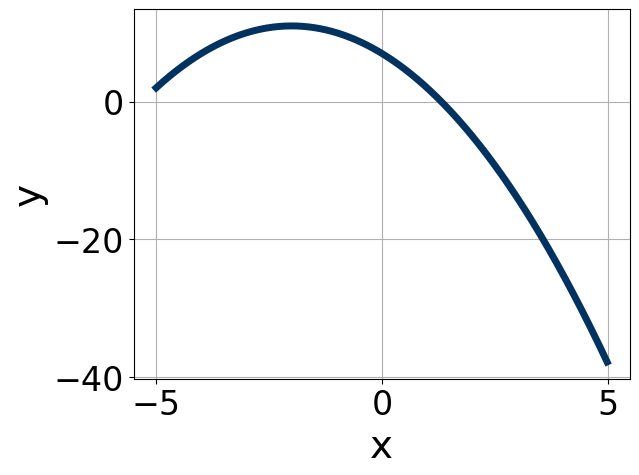
\includegraphics[width = 0.3\textwidth]{../Figures/quadraticEquationToGraphCC.png}\item 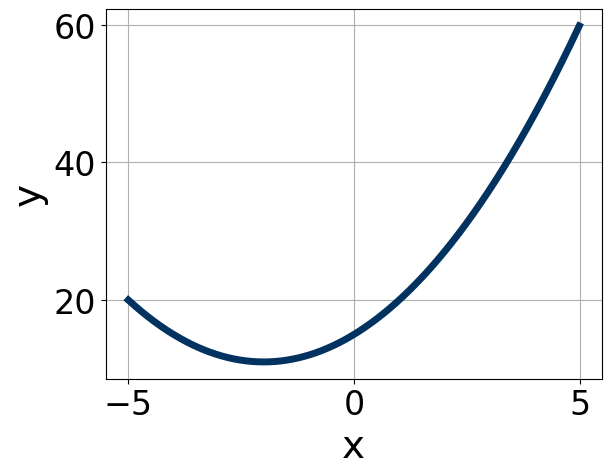
\includegraphics[width = 0.3\textwidth]{../Figures/quadraticEquationToGraphDC.png}\end{multicols}\item None of the above.
\end{enumerate} }
\litem{
Solve the quadratic equation below. Then, choose the intervals that the solutions $x_1$ and $x_2$ belong to, with $x_1 \leq x_2$.\[ 25x^{2} -60 x + 36 = 0 \]\begin{enumerate}[label=\Alph*.]
\item \( x_1 \in [0.07, 0.26] \text{ and } x_2 \in [5.1, 7.2] \)
\item \( x_1 \in [0.33, 0.56] \text{ and } x_2 \in [2.8, 4] \)
\item \( x_1 \in [0.93, 1.44] \text{ and } x_2 \in [0.9, 2] \)
\item \( x_1 \in [0.53, 0.83] \text{ and } x_2 \in [2.1, 2.8] \)
\item \( x_1 \in [29.93, 30.26] \text{ and } x_2 \in [29.6, 30.2] \)

\end{enumerate} }
\litem{
Solve the quadratic equation below. Then, choose the intervals that the solutions belong to, with $x_1 \leq x_2$ (if they exist).\[ -10x^{2} -7 x + 2 = 0 \]\begin{enumerate}[label=\Alph*.]
\item \( x_1 \in [-2.59, -2.04] \text{ and } x_2 \in [9.07, 10.05] \)
\item \( x_1 \in [-13.12, -11.38] \text{ and } x_2 \in [10.67, 11.15] \)
\item \( x_1 \in [-0.75, 0.18] \text{ and } x_2 \in [0.63, 1.43] \)
\item \( x_1 \in [-1.05, -0.78] \text{ and } x_2 \in [-0.47, 0.34] \)
\item \( \text{There are no Real solutions.} \)

\end{enumerate} }
\litem{
Write the equation of the graph presented below in the form $f(x)=ax^2+bx+c$, assuming  $a=1$ or $a=-1$. Then, choose the intervals that $a, b,$ and $c$ belong to.
\begin{center}
    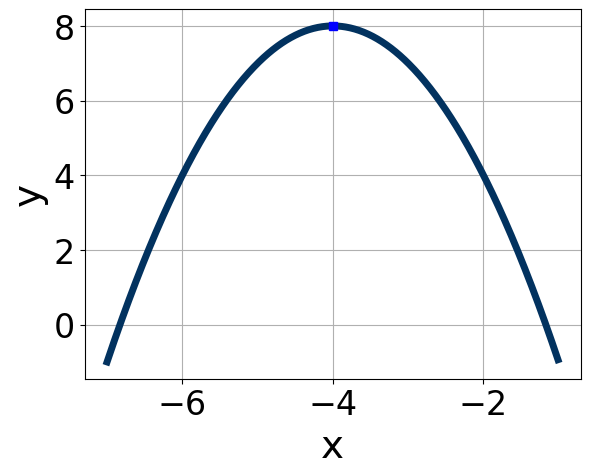
\includegraphics[width=0.5\textwidth]{../Figures/quadraticGraphToEquationCopyC.png}
\end{center}
\begin{enumerate}[label=\Alph*.]
\item \( a \in [-2, 0], \hspace*{5mm} b \in [5, 12], \text{ and } \hspace*{5mm} c \in [-9, -7] \)
\item \( a \in [-2, 0], \hspace*{5mm} b \in [-8, -7], \text{ and } \hspace*{5mm} c \in [-9, -7] \)
\item \( a \in [-2, 0], \hspace*{5mm} b \in [5, 12], \text{ and } \hspace*{5mm} c \in [-24, -18] \)
\item \( a \in [1, 2], \hspace*{5mm} b \in [-8, -7], \text{ and } \hspace*{5mm} c \in [21, 28] \)
\item \( a \in [1, 2], \hspace*{5mm} b \in [5, 12], \text{ and } \hspace*{5mm} c \in [21, 28] \)

\end{enumerate} }
\litem{
Factor the quadratic below. Then, choose the intervals that contain the constants in the form $(ax+b)(cx+d); b \leq d.$\[ 36x^{2} +37 x -10 \]\begin{enumerate}[label=\Alph*.]
\item \( a \in [2, 3.3], \hspace*{5mm} b \in [-4, 0], \hspace*{5mm} c \in [11.51, 12.51], \text{ and } \hspace*{5mm} d \in [5, 11] \)
\item \( a \in [14.6, 18.7], \hspace*{5mm} b \in [-4, 0], \hspace*{5mm} c \in [1.12, 2.35], \text{ and } \hspace*{5mm} d \in [5, 11] \)
\item \( a \in [6.4, 9.6], \hspace*{5mm} b \in [-4, 0], \hspace*{5mm} c \in [3.3, 4.64], \text{ and } \hspace*{5mm} d \in [5, 11] \)
\item \( a \in [-0.7, 2.2], \hspace*{5mm} b \in [-8, -4], \hspace*{5mm} c \in [0.62, 1.09], \text{ and } \hspace*{5mm} d \in [40, 50] \)
\item \( \text{None of the above.} \)

\end{enumerate} }
\litem{
Factor the quadratic below. Then, choose the intervals that contain the constants in the form $(ax+b)(cx+d); b \leq d.$\[ 54x^{2} -57 x + 10 \]\begin{enumerate}[label=\Alph*.]
\item \( a \in [16, 20], \hspace*{5mm} b \in [-8, -4], \hspace*{5mm} c \in [1.1, 3.8], \text{ and } \hspace*{5mm} d \in [-8, -1] \)
\item \( a \in [2, 4], \hspace*{5mm} b \in [-8, -4], \hspace*{5mm} c \in [15.3, 18.3], \text{ and } \hspace*{5mm} d \in [-8, -1] \)
\item \( a \in [-1, 2], \hspace*{5mm} b \in [-47, -41], \hspace*{5mm} c \in [-1.5, 1.3], \text{ and } \hspace*{5mm} d \in [-12, -9] \)
\item \( a \in [4, 8], \hspace*{5mm} b \in [-8, -4], \hspace*{5mm} c \in [6.7, 12.2], \text{ and } \hspace*{5mm} d \in [-8, -1] \)
\item \( \text{None of the above.} \)

\end{enumerate} }
\litem{
Solve the quadratic equation below. Then, choose the intervals that the solutions belong to, with $x_1 \leq x_2$ (if they exist).\[ 17x^{2} +9 x -3 = 0 \]\begin{enumerate}[label=\Alph*.]
\item \( x_1 \in [-17.47, -16.76] \text{ and } x_2 \in [16.34, 17.07] \)
\item \( x_1 \in [-0.3, 0.67] \text{ and } x_2 \in [0.59, 1.42] \)
\item \( x_1 \in [-13.31, -12.64] \text{ and } x_2 \in [3.72, 4.19] \)
\item \( x_1 \in [-0.82, -0.57] \text{ and } x_2 \in [-0.77, 0.32] \)
\item \( \text{There are no Real solutions.} \)

\end{enumerate} }
\end{enumerate}

\end{document}